\documentclass{article} % For LaTeX2e
\usepackage{nips12submit_e,times}
%\documentstyle[nips12submit_09,times,art10]{article} % For LaTeX 2.09
%\newtheorem{observation}{Observation}
%\newtheorem{claim}{Claim}
%\newtheorem{conjecture}{Conjecture}
%\newtheorem{problem}{Problem}
%\newtheorem{algo}{Algorithm}
%\newtheorem{definition}{Definition}
%\newtheorem{lemma}{Lemma}
%\newtheorem{theorem}{Theorem}
%\newtheorem{proof}{Proof}
%\newtheorem{defi}{Definition}

\newcommand\independent{\protect\mathpalette{\protect\independenT}{\perp}}
\def\independenT#1#2{\mathrel{\setbox0\hbox{$#1#2$}%
\copy0\kern-\wd0\mkern4mu\box0}} 

\newcommand{\atiter}[2]{{#1}^{(#2)}}
\newcommand{\itert}[1]{{#1}^{(t)}}
\newcommand{\itertO}[1]{{#1}^{(t+1)}}
\newcommand{\iiter}[1]{{#1}^{(i)}}
% \newcommand{\raiseTheta}[1]{\theta^{#1}}
\newcommand{\raisePsi}[1]{\psi^{#1}}
\newcommand{\order}[1]{\mathcal{O}(#1)}

\newcommand{\hide}[1]{}
\newcommand{\comment}[1]{\textcolor{red}{{\small #1 }}}
\newcommand{\semihide}[1]{{\tiny #1}}
\newcommand{\reminder}[1]{{\textsf{\textcolor{red}{[#1]}}}}
\newcommand{\makeclean}{
    \renewcommand{\reminder}[1]{}
}

%\newcommand{\QED}{ \hfill {\bf QED}}
\newcommand{\tight}{ \setlength{\itemsep}{-1.0\itemsep} }
    % makes lists tighter

\usepackage[mathscr]{eucal} %% For \mathscr
\usepackage{amsbsy} %% For \boldsymbol
\newcommand{\tensor}[1]{\boldsymbol{\mathscr{#1}}}   %% Tensor macro from Tammy
% \newcommand{\tensor}[1]{{\boldmath\mathcal{#1}}}
\newcommand{\B}[1]{\mathbf{#1}}   %% Tensor macro from Tammy
%\newcommand{\tensor}[1]{\underline{\mathbf{#1}}}  
%\newcommand{\tensor}[1]{\mathbf{\EuScript{#1}}}  
%\newcommand{\tensor}[1]{\mathbf{\mathcal{#1}}}  
\newcommand{\loss}{\mathcal{L}}  

\newcommand{\krp}[2]{ \left( \mathbf{#1}\odot\mathbf{#2} \right)}

\def\blambda{\mbox{\boldmath ${\lambda}$}}

\newcommand{\method}{\textsc{METHOD}\xspace}
\newcommand{\methodplain}{METHOD\xspace}
\newcommand{\graphlab}{GraphLab\xspace}
\newcommand{\psgd}{PSGD\xspace}
\newcommand{\dsgd}{DSGD+\xspace}
\newcommand{\lda}{LDA\xspace}
\newcommand{\dl}{DL\xspace}
\newcommand{\mmsb}{MMSB\xspace}
\newcommand{\twitter}{TGraph\xspace}
\newcommand{\nytimes}{NyTimes\xspace}
\newcommand{\snytimes}[1]{NyTimes{#1}\xspace}
\newcommand{\scaleblenytimes}{Scalable NyTimes\xspace}
\newcommand{\pubmed}{PubMed\xspace}
\newcommand{\imagenet}{ImageNet\xspace}

\newcommand{\sgd}{SGD\xspace}

%\newcommand{\explosion}{\textsc{Idex}\xspace}
\newcommand{\explosion}{intermediate data explosion\xspace}
\newcommand{\Explosion}{Intermediate Data Explosion\xspace}
\newcommand{\gtscaleup}{100\xspace}

\newcommand{\samplecube}{\textsc{ParCube}\xspace}
\newcommand{\parafac}{\textsc{Parafac}\xspace}
\newcommand{\sparafac}{\textsc{Parafac SLF}\xspace}
\newcommand{\merge}{\textsc{Merge}\xspace}
\newcommand{\sample}{\textsc{BiasedSample}\xspace}
\newcommand{\enron}{\textsc{Enron}\xspace}
\newcommand{\facebook}{\textsc{Facebook}\xspace}
\newcommand{\lbnl}{\textsc{Lbnl}\xspace}
\newcommand{\nell}{\textsc{Nell}\xspace}
\newcommand{\argmin}{\text{argmin}\xspace}
\newcommand{\brain}{\textsc{BrainQ}\xspace}


\newcommand{\hadi}{{\cal HADI}\xspace}
\newcommand{\mapreduce}{\textsc{MapReduce}\xspace}
\newcommand{\map}{\textsc{Map}\xspace}
\newcommand{\reduce}{\textsc{Reduce}\xspace}
\newcommand{\combine}{\textsc{Combine}\xspace}
\newcommand{\hadoop}{\textsc{Hadoop}\xspace}
\newcommand{\anf}{\emph{Centralized Method}}
% \newcommand{\MFB}{{MF-bitstring}}
\newcommand{\MFB}{{FM-bitstring}}
\newcommand{\mfb}{{b}}
\newcommand{\MFV}{{FM-vector}}
\newcommand{\mfv}{{\bf v}}
% \newcommand{\mfbhi}{{MF-vector}}
\newcommand{\mfbhi}{{ b(h,i) }}
\newcommand{\Nhi}{N(h,i)}   % number of neighbors of $i$, within h hops or less
\newcommand{\NNhi}{ {\cal N}(h,i)} % SET of neighbors ....
\newcommand{\NNhhi}{ {\cal N}(h+1,i)} % SET of neighbors ....
\newcommand{\NNhj}{ {\cal N}(h,j)} % SET of neighbors ....
\newcommand{\hatmfbhi}{ $\hat{b}(h,i)$} %partial bitmask

\newcommand{\PassA}{{\tt Stage1}\xspace}
\newcommand{\PassAMap}{{\tt Stage1-Map}\xspace}
\newcommand{\PassARed}{{\tt Stage1-Reduce}\xspace}
\newcommand{\PassB}{{\tt Stage2}\xspace}
\newcommand{\PassBMap}{{\tt Stage2-Map}\xspace}
\newcommand{\PassBRed}{{\tt Stage2-Reduce}\xspace}
\newcommand{\PassC}{{\tt Stage3}\xspace}
\newcommand{\PassCMap}{{\tt Stage3-Map}\xspace}
\newcommand{\PassCRed}{{\tt Stage3-Reduce}\xspace}

\newcommand{\diameter}{{\tt diameter}}
\newcommand{\npairs}{{\tt npairs}}
\newcommand{\gcc}{{\tt gcc}}
\newcommand{\entropy}{{\tt entropy}}
% \newcommand{\nedges}{{\tt nedges}}
\newcommand{\sv}{{\mbox{$\lambda_1$}}}
\newcommand{\avgd}{{\tt avgd}}

% math symbol definitions
\newcommand{\mat}[1]{{\bf{#1}}}
\newcommand{\nnodes}{N}     % number of nodes
\newcommand{\nedges}{E}     % number of edges
\newcommand{\deff}{{d_{eff}}}   % effective diameter
\newcommand{\Er}{{E_{r}}}   % number of retained edges
\newcommand{\Nr}{{N_{r}}}   % number of retained nodes
\newcommand{\Nc}{{N_c}}   % number of nodes at critical point
\newcommand{\Ec}{{E_c}}   % number of nodes at critical point
\newcommand{\Ngcc}{{N_{gcc}}} % number of nodes in gcc, at critical poing
\newcommand{\NPairc}{{N_{NPAIRS}}} % number of reachable pairs, at critical poing
\newcommand{\dc}{{d_{c}}} % diameter at critical point
\newcommand{\Lambdac}{{\lambda_{c}}} % First eigenvalue at critical point
% \newcommand{\RED}{ {\em RED } } % random edge deletion
% \newcommand{\FED}{ {\em FED } } % friendly edge deletion
% \newcommand{\HED}{ {\em HED } } % hostile edge deletion
\newcommand{\join}{\texttt{combine2}}
\newcommand{\aggrnp}{\texttt{combineAll}}
\newcommand{\aggr}{\texttt{combineAll$_i$}}
\newcommand{\aggrsid}{\texttt{combineAll$_{E.sid}$}}
\newcommand{\assign}{\texttt{assign}}



\newcommand{\ben}{\begin{enumerate*}}
\newcommand{\een}{\end{enumerate*}}
\newcommand{\bit}{\begin{itemize*}}
\newcommand{\eit}{\end{itemize*}}

% shorthands
\newcommand{\citationsds}{{CITATIONS}}
\newcommand{\epinionsds}{{EPINIONS}}
\newcommand{\patentsds}{{PATENTS}}
\newcommand{\net}[1]{{\textsc{#1}}}

\newcommand{\QED}{\hfill $\Box$ \hfill}





% graph segment
% Notation macros
\newcommand{\G}{\ensuremath{{\mathcal G}}}  % graph stream
\newcommand{\ES}[1]{\ensuremath{m^{(\!#1\!)}}}
%\newcommand{\ES}[1]{\ensuremath{|E|^{(\!#1\!)}}}
\newcommand{\coll}{\ensuremath{\ell}}  % number of source/row groups
\newcommand{\rowk}{\ensuremath{k}}  % number of dest/col groups
\newcommand{\rgrp}[1]{\ensuremath{I^{(\!#1\!)}}}  % node set for src/row group
\newcommand{\cgrp}[1]{\ensuremath{J^{(\!#1\!)}}} % node set for dst/col group
\newcommand{\rgsz}[1]{\ensuremath{l^{(\!#1\!)}}}  % size of node set for src/row group
\newcommand{\cgsz}[1]{\ensuremath{n^{(\!#1\!)}}  }% size of node set for dst/col group
\newcommand{\subG}[1]{\ensuremath{{\mathcal G}^{(\!#1\!)}}}  % submatrices
\newcommand{\den}[1]{\ensuremath{\rho^{(\!#1\!)}}}   % density/probability
\newcommand{\KL}[2]{\ensuremath{{\mathcal D}(#1\|#2)}}   % KL-divergence
\newcommand{\ceil}[1]{\ensuremath{\lceil\!#1\!\rceil}}   % density/probability

\newcommand{\myrot}[1]{\rotatebox[origin=ll]{75}{{#1}}} 


\usepackage{amsmath}%,amsthm}
\usepackage{amsfonts}
\usepackage{amssymb}
\usepackage{subfigure, fink, grffile, placeins}
\usepackage[pdftex]{graphicx} 
\usepackage{epstopdf}
\usepackage{hyperref}
% \usepackage[colorlinks,pagebackref]{hyperref}
% \usepackage[pagebackref]{hyperref}
\usepackage[usenames,dvipsnames]{xcolor}
%\usepackage{algorithmicx,algpseudocode,algorithm}
\usepackage{algorithm2e}
\usepackage{url}
% \usepackage[boxed,noend]{algorithm2e}
%\usepackage{mdwlist}    % from christos / mary: makes lists tighter
%\usepackage{epsfig}
%\usepackage{times}
%\usepackage{setspace}
%\usepackage[pdftex]{graphicx}
%\usepackage[pdftex]{geometry}

%\usepackage{algorithm}
%%\usepackage{algorithmic}
%\usepackage{algpseudocode}
%\usepackage{program}


\newtheorem{observation}{Observation}
\newtheorem{conjecture}{Conjecture}
\newtheorem{problem}{Problem}
\newtheorem{algo}{Algorithm}
\newtheorem{definition}{Definition}
\newtheorem{lemma}{Lemma}
\newtheorem{theorem}{Theorem}
%\newtheorem{question}{Question}
\newtheorem{example}{Example}
\newcommand{\pushright}[1]{\ifmeasuring@#1\else\omit\hfill$\displaystyle#1$\fi\ignorespaces}
\newcommand{\pushleft}[1]{\ifmeasuring@#1\else\omit$\displaystyle#1$\hfill\fi\ignorespaces}
%\newtheorem{answer}{Answer}
%\newtheorem{proof}{Proof}

\newcommand{\abhi}[1]{\textcolor{orange}{abhi-comment: #1}}
\newcommand{\alex}[1]{\textcolor{red}{\\ alex-comment: #1}}
\newcommand{\qirong}[1][1]{\textcolor{fuschia}{\\ qirong-comment: #1}}
\newcommand{\eric}[1][1]{\textcolor{blue}{\\ eric-comment: #1}}

\title{Slow-learner ain't My Problem: Exploiting Structure in
high-D, high-V Latent Space Stochastic Learning}
% \title{Community Discovery through Optimization}


\author{
% Abhimanu Kumar~~~~~~Alex Beutel~~~~~~Qirong Ho~~~~~~Eric P. Xing 
% \\ School of Computer Science, Carnegie Mellon University 
% \\ Pittsburgh PA 15213,USA,\\
% \{\href{mailto:abhimank@cs.cmu.edu}{abhimank},\href{mailto:abeutel@cs.cmu.edu}{abeutel},
% \href{mailto:qho@cs.cmu.edu}{qho},
% \href{mailto:epxing@cs.cmu.edu}{epxing}\}@cs.cmu.edu
}


% \authorrunning{Kumar et al.}
% The \author macro works with any number of authors. There are two commands
% used to separate the names and addresses of multiple authors: \And and \AND.
%
% Using \And between authors leaves it to \LaTeX{} to determine where to break
% the lines. Using \AND forces a linebreak at that point. So, if \LaTeX{}
% puts 3 of 4 authors names on the first line, and the last on the second
% line, try using \AND instead of \And before the third author name.

\newcommand{\fix}{\marginpar{FIX}}
\newcommand{\new}{\marginpar{NEW}}

\nipsfinalcopy % Uncomment for camera-ready version

\begin{document}


\maketitle

\begin{abstract}
	We pesent here a scheme for exploiting distributable structure present in
	latent space model for high-dimensional (high-D) and high-volume (high-V)
	learning. Models like latent dirichlet allocation, mixed membership
	stochastic blockmodels, dictionary learning have structures that can be
	exploted for big learning.
	We present a distributed learning strategy for such models. The scheme is
	distributed in data as well as parameter space and avoids waiting for slow
	learners to obtain full distributive leverage.
	The learning scheme, flexible to slow worker-processors, has
	provably correct strategy for convergence even with fewer synchronizations.
	It provides a tunable synchronization startegy that can be set based on the
	learning needs and system quality with the end user. We provide theoretical
	bounds on the parameter variance among workers with different synchronization 
	strategies. Empirical
	results presented for latent space models such as latent dirichlet allocation 
	and dictionary learning show that it scales very well with large data
	as well as parameter space. The comparative evaluation with other parallel
	and distributed learning startegies shows better preformance of the model.
	
\end{abstract}

\section{Introduction}
In todays information age there is trillions of bytes of data being generated
every moment. By one estimate we generate 5 exabytes of data on the internet every two
days~\footnote{\url{http://techcrunch.com/2010/08/04/schmidt-data/}} 
and most of
it is user generated content. Given this massive amount of data generated
every moment large scale machine learning is not just of academic
interest anymore but of practical significance too. Large scale learning or big
learning has been an active area of research in recent times. But most of this
research has been focused around big data and the aspect of distibuting the
learnig model has take back seat. While dealing with big data is definitely a must in this massive
content generation age the learning task might turn out to be non-trivial when
big data meets complex models. Learning models with high dimension or number of
parameters becomes non-trivial even with slight increase in data. 
Hence there is a need for learning scheme which can perform distributed data as
well as parameter learning. This problem is highly prevalent in latent space 
model such as latent dirichlet allocation (LDA~\cite{Blei:2003:LDA}), mixed
membership stochastic blockmodels (MMSB~\cite{Airoldi:2008:MMS}) as they inflate
their parameter space by introducing large number of latent variables.
Henceforth these models would be our object of focus in this paper. We develop a
stochastic learning scheme for latent space model, specifically for LDA and
MMSB, which is distributed in data as well as parameter space. We modify the
originial objective to suit our optimization scheme.\comment{need to write this
in a better way}. The structure obtained can be further exploited to minimize
the hazardous effects of slow-processors in the distributed system.  

\comment{expand some more giving an over view of our learning scheme}
\section{Related Work}
\comment{PSGD (only data parallel); Aggarawal and Duci's Distributed Delayed
(Again Data partition only; and it's hard to code); Any Other?}
\comment{How do we discuss the original Haas's paper though we do considerable
more in terms of theory and multi-iteration}
\comment{Theory work: Stochastic Approximation book; Zinkevich, Noboru Murata}

\section{Slow-learner Agnostic Distributed Learning Framework}

Our approach is to exploit independent cliques of structure present in large
scale machine learning models. Probabilistic graphical models introduce massive
amount of latent variables to induce the modelers belief regarding the
generative process of the data. Though this enables these models with a unique
ability to provide an interpretation and a generative story, it also makes the
model harder to learn since the parameter as well as variable space increases
massively. These models when run on large data have their learning problem
become twice difficult. 

While it may appear that latent space models' biggest boon
of incorporating hidden variables is their biggest bane for large scale
learning, it turns out that is not the case. On close examination it appears
that these latent variables have another adavantage: they have a structure. They
generally have cliques of correlated variable sets. This independence
structure can be exploited effectively for a distributed learning framework.
Moreover in models such as LDA and MMSB with a modified objective \comment{need to
put it in a better way} one can achieve distributivity in data as well as
parameters. We explain this using a basic LDA model. In simple terms, the aim of
an LDA model given a \emph{ document by vocabulary} matrix ($Y$) is to split it
into two matrices: a \emph{ documents by topics} ($\pi$, variable set) and
a \emph{ topics by vocabulary}  matrix ($\beta$, parameter set).
Equation~\ref{eqn:LDA} presents this in an optimization framework with simplex 
and non-negativity constraints. This is an
$\ell_p$ norm which is typecally $\ell_2$.
\begin{eqnarray}
\argmin_{\pi,\beta}L=||Y-\pi\beta||_p^p = \sum_{i,j}(Y_{i,j}-\sum_k
\pi_{i,k}\beta_{j,k})_p^p \label{eqn:LDA}\\
s.t.\sum_k\pi_{i,k}=1,\sum_k\beta_{j,k}=1, \pi_{i,k}\geq 0,
\beta_{j,k}\geq 0~~\forall~ i,j 
\nonumber
\end{eqnarray} 

For MMSB a similar objective can be formulated. Given a \emph{ user by user}
interaction strength %\comment{is it the right term} 
matrix $Y$ it aims to find
two matrices $\pi$ and $B$, which are \emph{user by topic} and \emph{topic by
topic} matrix respectively, such that $\pi^TB\pi$ reconstructs the original
matrix interaction matrix $Y$. Equation~\ref{eqn:MMSB} presents this in an
optimization framework with the usual non-negativity and simplex constraints. 

\begin{eqnarray}
\argmin_{\pi,B}L=||Y-\pi^TB\pi||_p^p = \sum_{i,j}(Y_{i,j}-\sum_{g,h}
\pi_{i,g}B_{g,h}\pi_{j,h})_p^p \label{eqn:MMSB}\\
s.t.\sum_k\pi_{i,k}=1,\pi_{i,k}\geq 0, B_{i,k}\geq 0~~\forall~ i,j \nonumber
\end{eqnarray}

For Dictionary Learning~\cite{Kreutz-Delgado:2003:DLA} the objective is
\begin{align}
\argmin_{\alpha,D} L=\frac{1}{2}||Y-D\alpha||_2^2 + \lambda||\alpha||_1
\label{eqn:dictionary}\\
s.t.~D_j^TD_j \leq 1 \forall j \nonumber
\end{align}
where $D$ is the dictionary being learnt and $\alpha$ is the sparse
representation of the signal
%  \comment{Do we present the symmetric matrix
% factorization objective too; since it's is nice scheduling scheme 
% as well as $\ell_p$ and $\ell_2$ combined loss}

For the LDA objective, figure~\ref{fig:para-div} shows the way parameters and
variable sets are divided in the distributive scheme. 
The distinction between parameter and variables comes in the projection step.
While the simplex projection for variables set ($\pi$) is done at each
update iteration i.e. each SGD update, the simplex projection for the parameters
in LDA is done at synchronization with other workers. We perform
parameter/variable updates of different blocks parallely. For SGD we perform
updates for $\mathbf{\pi, \beta}$, which we will collectively refer to as 
$\bold{\Psi}$ matrix whereas $\psi$ are the individual components of the matrix.
This definition of $\bold{\Psi}$ and $\psi$ will come in handy for updates to
variable or parameters based on the gradient at individual data points. 
E.g. the update for the LDA objective $L$ are: 
%(\comment{note:projections are involved here})
\begin{align}
\psi^{(t+1)}&= \psi^{(t)} - \eta_t \nabla
\loss_{Y_{i,j}}(\psi^{(t)})
\label{equ:sgd-update-lda}
\end{align}
Appropriate projections are applied to after the step in equation~\ref{equ:sgd-update-lda}
based on whether the updated value is of a parameter or a variable.  
\begin{figure}
\begin{center}
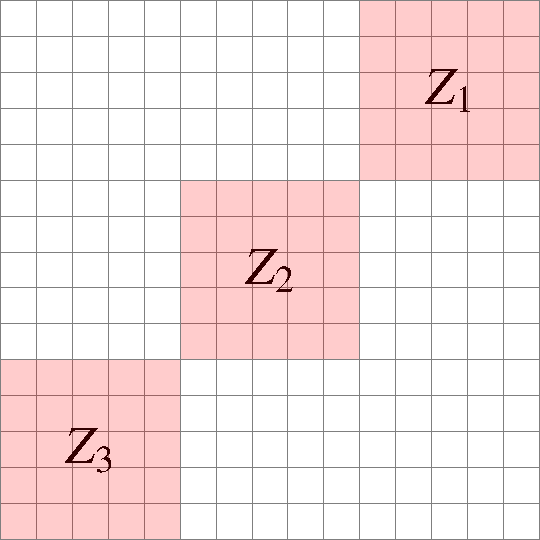
\includegraphics[width=0.2\textwidth]{fig/2dblocks.pdf}
\vspace{-4mm}
\caption{Dividing the \emph{document by vocabulary} matrix fo LDA into blocks
such that no two of them share any row or a column.}
\end{center}
\label{fig:para-div}
\end{figure}

For these update rules, we list below the differentials for each component
$\sigma$ of $\psi$ where norm use is $\ell_2$, and $(\nabla
L_{Y_{i,j}}(\psi))_\sigma = \frac{\partial L_{Y_{i,j}}}{\partial \sigma}$:
\begin{align}
	(\nabla L_{Y_{i,j}}(\psi))_\sigma &= 
	\left\{
	\begin{array}{ll}
		-2(Y_{i,j}-\sum_r \pi_{i,r}\beta_{j,r}
		)\beta_{j,\ell}  & \mbox{if } \sigma = \pi_{i,\ell} \\
		0 & \mbox{if } \sigma = \pi_{i',\ell},\ i\neq i'\\
	\end{array}
	\label{eqn:diff-lda}
\right.
\end{align}
similarly for $\sigma=\beta_{j,l}$. 
From this we observe that SGD update for $\pi_{i,l}$ at a particular entry
$Y_{i,j}$ depends only on previous $\pi_{i,r},
\beta_{j,r}$ where $r\in {1,\ldots,R}$ and $R$ is the number of topics we chose.
The updates for each component are similar for the MMSB case. 
%\comment{modify here for MMSB}

\begin{algorithm}
Input : $Y,\beta, \pi$,~sub-epoch~size~$d$\\
$\pi\leftarrow \pi_0$, $\beta\leftarrow \beta_0$\\
Block $Y,\pi,\beta$ into corresponding $w$ blocks\\
\While{not converged}{
Pick step size $\eta_S$\\
% 	\For{$s=0,...,d^2-1$}{
%		\\\*sub-epoch\*\\\\
		Pick $w$ blocks($S_{1},...,S_{w}$) to form sub-epoch $S$\\
		\For{$b=0,\ldots,w-1$ \textbf{in parallel}}{
			Run SGD on the training points $S_{b}$\\
			/\/** Do until every block is ready to synchronize **/\\\
			/\/** So potentially each block $S_{b}$ runs through each data-point
			multiple times if slow workers **/\\\
			Apply appropriate constraints (e.g. data-variable constraints in LDA).
		}
		Apply appropriate constraints (e.g. parameter constraints in LDA) 
% 	}
% \comment{add the fact that constraints sets applied can be different on
% parameter and data side} 
}
\caption{Algorithm for LDA updates. The $w$ blocks correspond to $w$ worker
processors}
\label{algo:lda}
\end{algorithm} 

Given this understanding of our optimization objective and SGD update rules, we
would like to segment our data in such a way that certain blocks $S_b$ can be
run in parallel, where we define $S_b \subseteq Y$.
Figure \ref{fig:para-div} shows the way we segment
our simple matrix $Y$ to enable parallelization. 
In order to run SGD on our blocks in parallel, we divide them such that no two
blocks share common rows or columns.  To be more precise, we say that a point
$y \in S_b$ is the coordinates in the data, such as $y = (y_i,y_jy) \in
Y$.  Two blocks $S_b$ and $S_{b'}$ are non-overlapping if
for all $y \in S_b$ and
$y' \in S_{b'}$, $y_i \neq y'_i$ and $y_j \neq y'_j$.
In order to cover all regions of
$Y$, we need multiple sub-epochs.
In our algorithm, we run the sub-epochs sequentially, but for each sub-epoch we
run SGD on the blocks in parallel. Different blocks in a sub-epoch can make
different number
of passes through the data. This is where the algorithm is robust against slow
processors as the worker keep running instead of waiting until every body is
ready to synchronize.   (Note, the order in 
which you run the sub-epochs does not matter, as long as they are each run once
per epoch.)  Algorithm \ref{algo:lda} explain the steps more formally.
We next offer a proof that this multi-iteration per block distributed
parameter learning converges appropriately. 





% \comment{Our Learning framework presented here. We present it in a way that
% emphasizes on latent space models\\} 
% \comment{Salient points: \\
% 1) different processors can make different number of iterations 
% over the data without synchronization. \\
% 2) The workers donot wait for slower workers and instead keep
% working and synchronize when everybody is ready. We should add that one
% can choose to not synchronize often based on how much they want variance among
% different processors and how slow is their slowest processor.\\
% 3) We present theoretical guaranties for convergence; **for simple as well
% as projected loss**\\
% 4) We provide bounds on variance among different workers at epoch and
% sub-epoch levels.\\
% 5) We demonstrate theoretically that keep doing work in place of waiting gets
% faster convergence. **TODO** \\
% % (Use potential energy tehnique) 
% 6) We show that our results are for generic loss fucntion and works
% even with projections/constraints($\ell1$, Non-negativity, Simplex etc.)\\
% 7) **Our assumptions: The structure; Martingale Diference Error $\varepsilon$}


\section{Theoretical Analysis}
\comment{\\ 1) Convergence (with projection)\\
2) Epoch variance bound\\
3) Sub-epoch variance bound\\
4) Show that waiting is not a good idea and workers should keep working till
every one is ready\\}

Here we analyse the method presented in algorithm~\ref{algo:lda} theoretically.
We will prove that the multi-iteration per block strategy converges. We
provide a bound on the variance accross two blocks with in a sub-epoch
running parallely. We show theoretically how the variance varies 
after each synchronization between two consecutive epochs. In the end we show
why working instead of wating for the slowest processor is a better strategy. 

\subsection{Convergence proof}
We introduce
$\atiter{V}{t}(\atiter{\psi}{t+1},\atiter{\psi}{t})$: a state potential
function that is defined over the past $\atiter{\psi}{t}$, future
$\atiter{\psi}{t+1}$ and the data points $\atiter{y}{t}$ picked at
iteration. $V^{(t)}$ encodes the probability of update in the parameter
from $\atiter{\psi}{t}$ to $\atiter{\psi}{t+1}$ through updating over a new
point $y^{(t)}$. We have the relation
\begin{equation}
p(\atiter{\psi}{t+1}|\atiter{\psi}{t}) d\atiter{\psi}{t} =
p(V^{(t)}(\atiter{\psi}{t+1},\atiter{\psi}{t}))
dV^{(t)}(\atiter{\psi}{t+1},\atiter{\psi}{t})
\label{eqn:potentialDef}
\end{equation}
$V^{(t)}(\atiter{\psi}{t+1},\atiter{\psi}{t})$ and
$dV^{(t)}(\atiter{\psi}{t+1},\atiter{\psi}{t})$ define the data points
picked and the volume element of this choice respectively, to get the new update
$\atiter{\psi}{t+1}$ from $\atiter{\psi}{t}$. 
% This is similar to probability
% rectangle defined in~\cite{Murata98astatistical}(appendix A.1) where we extend
% it to a collection of examples in later proofs.
$\itert{V}=\itert{V}(\itertO{\psi},\itert{\psi})$ can be understood as a 
fucntion that keeps track of the state of $\itert{\psi}$ and $\itertO{\psi}$ and depends
upon the data-point $\itert{Y_{i,j}}$ picked in the SGD update.

We define $ \nabla\mathcal{L}(\itert{\psi})$ as the exact gradient at iteration
$t$. We denote error at iteration $t$, $\left[
\nabla\mathcal{L}(\itert{\psi}) - \delta
\itert{L}(\itert{V},\itert{\psi})\right]$, as $\varepsilon_t$ where $\delta
\itert{L}(\itert{V},\itert{\psi})$ is the SGD gradient at iteration $t$ i.e.
$\nabla \loss_{Y_{i,j}}(\psi^{(t)})$.
We make the assumption that the error $\varepsilon_t=\left[
\nabla\mathcal{L}(\itert{\psi}) - \delta
\itert{L}(\itert{V},\itert{\psi})\right]$ in each step is a martingale
difference sequence. i.e we assume that 
\begin{eqnarray}
E\left[\nabla\mathcal{L}(\itert{\psi}) - \delta
\itert{L}(\itert{V},\itert{\psi})|\delta
\iiter{L}(\iiter{V},\iiter{\psi}),\iiter{\psi},i<t,\itert{\psi}\right] &=&
0 \nonumber \\
E\left[\varepsilon_t|\varepsilon_i,i<t\right] &=& 0
\label{eqn:martingaleAssumption}
\end{eqnarray} 
% \comment{Move the following justification of martingale sequence some where
% more relevant} 
We have to note here that assuming error terms are a martingale
difference sequence is a weaker assumption than assuming error terms
$\varepsilon_i$ are independent of each other. Making the martingale difference
assumption means that $\delta \itert{L}(\itert{V},\itert{\psi})$ conditioned on $\psi^{(0)}$ and $\delta
\iiter{L}(\iiter{V},\iiter{\psi}),i<n$, depends only on $\itert{\psi}$. 
This is achieved since the blocking strategy
explained earlier has no overlap between two parameters that are updated
parallely. 

We have $w$ worker processors (algorithm~\ref{algo:lda}) and assume that every
worker $i$ touches $n_i$ data point (with repeitition). In other words if the
worker $i$ was asigned $n$ points and it touches each point $\kappa_i,
\kappa_i\geq 1,$ times on an average in its block before syncing then we define
$n_i$ and $N_w$ as
\begin{align}
n_i = \kappa_i n\hspace{3cm}\text{and} && N_w = \sum_{i=1}^w n_i 
\label{eqn:workerIpoints}
\end{align}


\begin{theorem}
	The stochastic updates 
	$\psi^{(t+1)}= \psi^{(t)} - \eta_t \nabla \loss_{Y_{i,j}}(\psi^{(t)})$ as
	described in algorithm~\ref{algo:lda} and the exact updates
	$\psi^{(t+1)}=\itert{\psi} - \eta_t\nabla \mathcal{L}(\itert{\psi})$ (in case
	of an exact gradient descent) converge to the same set of limit points
	asymptotically, given that the error terms $\varepsilon_t$ are martingale
	difference sequence, $E[\varepsilon_t^2]<D$ (bounded variance) and
	$\sum\eta_i^2 <\infty$
	\label{theo:asymptotConverge}
\end{theorem}
\textbf{Proof.}

From equation~\ref{equ:sgd-update-lda} we have
\begin{eqnarray}
\itertO{\psi} &=& \itert{\psi} - \eta_t\delta
\itert{L}(\itert{V},\itert{\psi}) \nonumber\\ %\Longrightarrow \itertO{\psi} 
&=& \itert{\psi} - \eta_t\nabla
\mathcal{L}(\itert{\psi}) + \eta_t\left[ \nabla\mathcal{L}(\itert{\psi}) -
\delta \itert{L}(\itert{V},\itert{\psi})\right] \nonumber\\
 &=& \itert{\psi} - \eta_t\nabla
\mathcal{L}(\itert{\psi}) + \eta_t\varepsilon_t
\end{eqnarray} 
 
Using $n_i$ and $N_w$ as defined in equation~\ref{eqn:workerIpoints}

\begin{align}
\psi^{(t+(\sum_1^w n_i)m)} = \itert{\psi} + \sum_{i=t}^{t+m(\sum_1^w n_i)}
-\eta_i\mathcal{\nabla L}(\iiter{\psi}) +  \sum_{i=t}^{t+m(\sum_1^w n_i)}
\eta_i\varepsilon_i \nonumber\\
\Longrightarrow \psi^{(t+mN_w)} = \itert{\psi} + \sum_{i=t}^{t+mN_w}
-\eta_i\mathcal{\nabla L}(\iiter{\psi}) + \sum_{i=t}^{t+mN_w}
\eta_i\varepsilon_i \nonumber\\ 
\text{assuming~$\sum_1^w n_i=N_w$} \nonumber \\
\Longrightarrow \psi^{(t+mN_w)} = \itert{\psi} + \sum_{i=t}^{t+mN_w}
-\eta_i\mathcal{\nabla L}(\iiter{\psi}) + M_{mN_w}
\end{align}

where $M_{mN_w}=\sum_{i=t}^{t+mN_w} \eta_i\varepsilon_i$ is a martingale
sequence since it is a sum of martingale difference sequence. $mN_w$
captures the $m$ whole sub-epochs of work done as a whole by all the workers combined.
From Doobs martingale inequality (\cite{Friedman:1975}, ch. 1, Thm 3.8)
\begin{equation}
P\left(\sup_{t+mN_w\geq r \geq t}|M_r|\geq c\right) \leq \frac{E\left[\left(
\sum_{i=t}^{t+mN_w}\eta_i\varepsilon_i\right)^2\right]}{c^2}
\label{eqn:doobs}
\end{equation}

where $M_r=\sum_{i=t}^r\eta_i\varepsilon_i$. Lets look at the RHS of
equation~\ref{eqn:doobs} above:
\begin{align}
E\left[\left(\sum_{i=t}^{t+mN_w}\eta_i\varepsilon_i\right)^2\right] &=
E\left[\sum_{i=1}^{mN_w}\left(\eta_i\varepsilon_i\right)^2\right]
\nonumber\\\text{(equation~\ref{eqn:martingaleAssumption}
$\Longrightarrow~E[\varepsilon_i \varepsilon_j]=0$ if $i\neq j$)}\nonumber\\
=\sum_{i=1}^{mN_w}\eta_i^2E[\varepsilon_i^2] &\leq
\sum_{i=1}^{mN_w}\eta_i^2D \to 0 \nonumber\\
\text{where $E[\varepsilon_i^2]<D~\forall i$ and assuming $\sum\eta_i^2 <\infty$
} \nonumber\\ 
\lim_{t\to\infty}\Longrightarrow P\left(\sup_{i\geq t}|M_i|\geq c\right) =
0~~as~~t\to\infty
\label{eqn:asymptotoError}
\end{align}

From equation~\ref{eqn:asymptotoError} we have
\begin{align*}
\psi^{(t+mN_w)} = \itert{\psi} + \sum_{i=t}^{t+mN_w}
-\eta_i\mathcal{\nabla L}(\iiter{\psi})
% \label{eqn:asymptotConverge}
\end{align*}
asymptotically. Hence the algorithm converges to the same set of limit points as
the exact gradient descent asymptotically. Note that we do a theoretical
analysis of the algorithm without projection steps. Extending the proof to include 
projection can be done by using Arzela-Ascoli theorem and the limits of
converging sub-sequence of our algorithm's SGD updates~\cite{Kushner:yin}.

\hfill$\blacksquare$


\subsection{Intra sub-epoch variance}
We assume for simplicity that the parameter being updated in block-$i$ is univariate. 
This analysis can be
easily extended to a multivariate parameter updation case in each block of a
sub-epoch.
$\atiter{\psi}{t}$ is the value of parameter theta at iteration $t$. 
$\eta_t$ is the step size at iteration $t$ and
$\atiter{L}{t}$ is the loss at point $\atiter{y}{t}$ in iteration $t$. We define
$v^t=V^{(t)}$ the potential function defined at iteration $t$ as in
equation~\ref{eqn:potentialDef}


\begin{align}
\atiter{\psi}{t+1} = \atiter{\psi}{t} -
\delta\atiter{\psi}{t}(\atiter{V}{t},\atiter{\psi}{t}) 
\label{eqn:iterDelta1} \\
%\end{eqnarray}
\text{where 
$\,\delta\atiter{\psi}{t}(\atiter{V}{t}, \atiter{\psi}{t}) =
\atiter{\eta}{t}\delta\atiter{L}{t}(\atiter{V}{t},\atiter{\psi}{t})\Rightarrow
\raisePsi{(t+1)} = \raisePsi{t} - \eta_{t} \delta L^{t} \! (V^{t},
\raisePsi{t})$} \nonumber\\
\text{Summing equation~\ref{eqn:iterDelta1} over $n_i$, the number of points
updated in block $i$ of a sub-epoch} \nonumber\\
\raisePsi{t+n_{i}} = \raisePsi{t} - \sum_{i=1}^{n_{i}} \! \eta_{t+i} \delta
L^{t+i}(V^{t+i}, \psi^{t+i})
\end{align}

Let $V$ denote denote the joint potential for all the $n_i$ points encountered
in block $i$. The equation~\ref{eqn:potentialDef} can be extended as 

\begin{align}
p(\raisePsi{(t+n_i)}|\raisePsi{t}) d\raisePsi{(t+n_i)} &= 
p(V(\raisePsi{(t+n_i)}, \raisePsi{t})) dV \nonumber\\
\Rightarrow p(\raisePsi{(t+n_i)}) d\raisePsi{(t+n_i)}  
&= \int_{\raisePsi{t}} \!
p(\raisePsi{(t+n_i)}|\raisePsi{t}) p(\raisePsi{t}) d \raisePsi{t} 
d \raisePsi{(t+n_i)}
= \int_{\raisePsi{t}} \! p(V(\raisePsi{(t+n_i)}, \raisePsi{t})) dV 
p(\raisePsi{t}) d \raisePsi{t}
\label{eqn:newPotentialDef}
\end{align}



\begin{lemma}
	Let $u(\raisePsi{(t+n_i)})$ be a function of $\raisePsi{(t+n_i)}$ then
	
\begin{equation*}
\mathbb{E}^{\raisePsi{(t+n_i)}}[u(\raisePsi{(t+n_i)})] =
\mathbb{E}^{\raisePsi{t}}[\mathbb{E}^{V}[u(\raisePsi{(t+n_i)})]]
\end{equation*}
\label{theo:expectNewPsi}
\end{lemma}
\textbf{Proof.}
From equation~\ref{eqn:newPotentialDef}
\begin{align}
\mathbb{E}^{\raisePsi{(t+n_i)}}[u(\raisePsi{(t+n_i)})] &= 
\int_{\raisePsi{(t+n_i)}} \! u(\raisePsi{(t+n_i)}) p(\raisePsi{(t+n_i)}) d 
\raisePsi{(t+n_i)} \nonumber\\
&= \int_{\raisePsi{t+i}} 
\! u(\raisePsi{(t+n_i)}) P(\raisePsi{(t+n_i)}) d\raisePsi{(t+n_i)}\nonumber\\
&= \int_{V} \! \int_{\raisePsi{t}} \! u(\raisePsi{(t+n_i)}) P(V(\raisePsi{(t+n_i)}, \psi)) 
dV P(\raisePsi{t}) d\raisePsi{t}\nonumber\\
&= \mathbb{E}^{\raisePsi{t}}[\mathbb{E}^{V}[u(\raisePsi{(t+n_i)})]]
\nonumber
\end{align}
\hfill$\blacksquare$
\begin{lemma}
\begin{equation*}
\mathbb{E}^{V}[\delta L^{t+i} (v^{t+i}, \psi^{t+i})] =
\frac{d\mathbb{E}^{V}[L^{t+i} (v^{t+i}, \psi^{t+i})]}{d\psi^{t+i}}
\end{equation*}
\label{theo:derivativeExpect}
\end{lemma}
\textbf{Proof.}
Due to randomness in picking the point to be updated in iteration $t+i$ We have 
\begin{align*}
\mathbb{E}^{V}[L^{t+i} (v^{t+i}, \psi^{t+i})] &= \int L(y,\psi^{t+i}) dy\\ 
\Rightarrow \frac{d\mathbb{E}^{V}[L^{t+i} (v^{t+i},
\psi^{t+i})]}{d\psi^{t+i}} &=
\mathbb{E}^{V}[\frac{dL^{t+i} (v^{t+i},
\psi^{t+i})}{d\psi^{t+i}}]=\mathbb{E}^{V}[\delta L^{t+i} (v^{t+i}, \psi^{t+i})]
\end{align*}
\hfill$\blacksquare$

\begin{lemma}
\begin{equation*}
\mathbb{E}^{V}[L^{t+i}
(v^{t+i}, \psi^{t+i})] = \mathbb{E}^{v^{t+i}}[L^{t+1} (v^{t+i},
\psi^{t+i})]
\end{equation*}
\label{theo:independentPotentialExpectation}
\end{lemma}
\textbf{Proof.}

Using the definition of $V^{t+i}$ in equation~\ref{eqn:potentialDef}, the
fact that $V$ is a joint variable of each $V^{t+i}$  and an any
iteration $t+i$ the chance of picking any data point is completely random and
indpendent of any other iteration.
\begin{equation*}
\mathbb{E}^{V}[L^{t+i}
(v^{t+i}, \psi^{t+i})] = \mathbb{E}^{v^{t+i}}[L^{t+1} (v^{t+i},
\psi^{t+i})]
\end{equation*}
\hfill $\blacksquare$

\begin{lemma}
\begin{equation*}
\mathbb{E}^{V}[\frac{dL^{t+i} (v^{t+i},
\psi^{t+i})}{d\psi^{t+i}}\frac{dL^{t+j} (v^{t+j}, \psi^{t+i})}
{d\psi^{t+j}}] =\frac{d\mathbb{E}^{v^{t+i}}[L^{t+i}
(v^{t+i}, \psi^{t+i})]}{d\psi^{t+i}}\frac{d\mathbb{E}^{v^{t+i}}[L^{t+i} (v^{t+i},
\psi^{t+i})]}{d\psi^{t+i}}
\end{equation*}
\label{theo:independentPotentialCovariance}
\end{lemma}
\textbf{Proof.}
Two different data
points picked at iteration $(t+i)$ and $(t+j)$ are independent of each other.
Using this fact and the definition of potetntial function $V$ in
equation~\ref{eqn:newPotentialDef}
\begin{align*}
\mathbb{E}^{V}[\frac{dL^{t+i} (v^{t+i},
\psi^{t+i})}{d\psi^{t+i}}\frac{dL^{t+j} (v^{t+j}, \psi^{t+i})}
{d\psi^{t+j}}] &= \mathbb{E}^{V}[\frac{dL^{t+i} (v^{t+i},
\psi^{t+i})]}{d\psi^{t+i}}]\mathbb{E}^{V}[\frac{dL^{t+j} (v^{t+j},
\psi^{t+i})} {d\psi^{t+j}}] \\
\text{\bigg(using lemma~\ref{theo:derivativeExpect}\bigg)}& =
\frac{d\mathbb{E}^{V}[L^{t+i} (v^{t+i}, \psi^{t+i})]}{d\psi^{t+i}}
\frac{d\mathbb{E}^{V}[L^{t+j} (v^{t+j}, \psi^{t+j})]}{d\psi^{t+j}} \\
\text{\bigg(using lemma~\ref{theo:independentPotentialExpectation}\bigg)}& =
\frac{d\mathbb{E}^{v^{t+i}}[L^{t+i} (v^{t+i}, \psi^{t+i})]}{d\psi^{t+i}}
\frac{d\mathbb{E}^{v^{t+j}}[L^{t+j} (v^{t+j}, \psi^{t+j})]}{d\psi^{t+j}}
\end{align*}
\hfill $\blacksquare$

\begin{theorem}
We define $\psi_*$ as the global optima and $\Omega_0$ as the hessian of the
loss at $\psi_*$ i.e. $\Omega_0 = \frac{d^2\mathbb{E}[L(\psi_*)]}{d\psi_*^2}$
(assuming that $\psi$ is univariate) then
\begin{align*}
\frac{d\mathbb{E}^{v^{t+i}}[L^{t+i} (v^{t+i}, \psi^{t+i})]}{d\psi^{t+i}} =
\Omega_0(\psi_t-\psi_* + \delta_i) + \order{\rho_t^2}
\end{align*}
where $\order{\rho_t^2} = \order{|\psi_{t+i}-\psi_*|^2}$ with the assumption 
that $\order{\rho_{t+i}}$ is small $\forall i\geq 0$ and $\delta_i =
\psi_{t+i}-\psi_t$.
\end{theorem}
\label{theo:optimaGradient}
\textbf{Proof.}
Lets define $\phi(\psi_{t+i}) = \mathbb{E}^{v^{t+i}}[L^{t+i} (v^{t+i},
\psi^{t+i})]$ 
Using Taylor's theorem and expanding around $\psi_*$
\begin{align*}
\phi(\psi^{t+i}) = \phi(\psi_*) + \frac{d\phi(\psi_*)}{d\psi_*}
(\psi^{t+i}-\psi_*) + \frac{(\psi^{t+1}-\psi_*)^2}{2}
\frac{d^2\phi(\psi_*)}{d\psi_*^2} + \order{(\psi^{t+i}-\psi_*)^3}\\
= \phi(\psi_*) + \frac{(\psi^{t+i}-\psi_*)^2}{2}
\frac{d^2\phi(\psi_*)}{d\psi_*^2} + \order{(\psi^{t+i}-\psi_*)^3}
\,\text{\bigg(as $\frac{d\phi(\psi_*)}{d\psi_*} = 0$ at optima\bigg) } \\
\Rightarrow \frac{d\phi(\psi^{t+i})}{d\psi^{t+i}} =
(\psi^{t+i}-\psi_*)\frac{d^2\phi(\psi_*)}{d\psi_*^2} +
\order{(\psi^{t+i}-\psi_*)^2} \\
\Rightarrow \frac{d\mathbb{E}^{v^{t+i}}[L^{t+i} (v^{t+i},
\psi^{t+i})]}{d\psi^{t+i}} = \Omega_0(\psi^t-\psi_* + \delta_i) +
\order{\rho_t^2} \text{\bigg( with the assumption that $\order{\rho_t}$ is
small} \\ \text{we have $\order{\rho_{t+i}^2} = \order{\rho_t^2} $ 
\bigg)}
\end{align*}
\hfill $\blacksquare$

\begin{theorem}
With $\psi_*$ as defined in theorem~\ref{theo:optimaGradient} and assuming that $\psi$ is 
univariate we have
\begin{align*}
\mathbb{E}^{v^{t+i}}[(\frac{dL^{t+i} (v^{t+i},
\psi^{t+i})} {d\psi^{t+i}})^2] = \Omega_1 +
\order{\mathbb{E}[\order{\rho_t}]} + \order{\rho_t^2}
\end{align*}
where $\order{\rho_t^2}$ and $\delta_i$ are as defined
in theorem~\ref{theo:optimaGradient} and $\Omega_1=\mathbb{E}^{v^{t+i}}[
(\frac{dL^{t+i}(v^{t+i},\psi_*)}{d\psi_*})^2]$
\label{theo:optimaGradientSquare}
\end{theorem}
\textbf{Proof.}
Expanding $L^{t+i} (v^{t+i},\psi^{t+i})$ around $\psi_*$ using Taylor's
theorem 
\begin{align*}
L^{t+i} (v^{t+i},\psi^{t+i}) = L^{t+i} (v^{t+i},\psi_*) + \frac{dL^{t+i}
(v^{t+i},\psi_*)}{d\psi_*}(\psi^{t+i}-\psi_*) \\
+ \frac{1}{2}\frac{d^2L^{t+i}
(v^{t+i},\psi_*)}{d\psi_*^2}(\psi^{t+i}-\psi_*)^2 +
\order{(\psi^{t+i}-\psi_*)^3}\\
\Rightarrow \frac{dL^{t+i} (v^{t+i},\psi^{t+i})} {d\psi^{t+i}} = \frac{dL^{t+i}
(v^{t+i},\psi_*)}{d\psi_*} + \frac{d^2L^{t+i}
(v^{t+i},\psi_*)}{d\psi_*^2}(\psi^{t+i}-\psi_*) + \order{(\psi^{t+i}-\psi_*)^2}
\\
\Rightarrow \mathbb{E}^{v^{t+i}}[(\frac{dL^{t+i} (v^{t+i},\psi^{t+i})}
{d\psi^{t+i}})^2] = \mathbb{E}^{v^{t+i}}[
(\frac{dL^{t+i}(v^{t+i},\psi_*)}{d\psi_*})^2  \\+ 2
\frac{dL^{t+i}(v^{t+i},\psi_*)}{d\psi_*} \frac{d^2L^{t+i}
(v^{t+i},\psi_*)}{d\psi_*^2}(\psi^{t+i}-\psi_*) +
\order{(\psi^{t+i}-\psi_*)^2}]\\
\Rightarrow \mathbb{E}^{v^{t+i}}[(\frac{dL^{t+i} (v^{t+i},
\psi^{t+i})} {d\psi^{t+i}})^2] = \Omega_1 +
\order{\mathbb{E}[(\psi_{t+i}-\psi_*]} + \order{\rho_t^2}\\
= \Omega_1 +
\order{\mathbb{E}[\order{\rho_t}]} + \order{\rho_t^2}
\end{align*}
\hfill $\blacksquare$

\begin{theorem}
The variance of the parameter $\psi$ at the end of a sub-epoch $S$ in block
$S_i$ which updated $n_i$ points as defined in equation~\ref{eqn:workerIpoints}
is
\begin{align*}
Var(\raisePsi{t+n_i}) &= Var(\psi^t)- 2\eta_tn_i\Omega_0(Var(\psi^t))
-2\eta_tn_i\Omega_0CoVar(\psi_t,\bar{\delta_t}) + \eta_t^2n_i\Omega_1 \nonumber\\ 
&+ \underbrace{\order{\eta_t^2\rho_t} +
\order{\eta_t\rho_t^2} +
\order{\eta_t^3}+ \order{\eta_t^2\rho_t^2}}_{\Delta_t}
\end{align*}
Constants $\Omega_0$ and $\Omega_1$ are defined in
theorems~\ref{theo:optimaGradient} and theorems~\ref{theo:optimaGradientSquare}
respectively. 
\end{theorem}
\textbf{Proof.}
We start with analysing $\mathbb{E}^{V}[u(\psi^{(t+ni)})]$ term from
lemma~\ref{theo:expectNewPsi}
\begin{align}
&\mathbb{E}^{V}[u(\psi^{(t+ni)})] = \mathbb{E}^{V}[u(\psi^{t} +
(-\underbrace{\sum_{i=1}^{n_{i}} \! \eta_{t+i} \delta L^{t+i} (v^{t+i},
\psi^{t+i})}_{\nabla}))] \nonumber\\
& = \mathbb{E}^{V}[u(\psi^{t}) - \frac{du(\psi^{t})}{d\psi^{t}}\nabla +
\frac{1}{2}\frac{du^2(\psi^{t})}{d(\psi^{t})^2}\nabla^2 + \order{\eta_t^3}]
\nonumber\\
& = u(\psi^{t}) -
\eta_t\frac{du(\psi^{t})}{d\psi^{t}}\mathbb{E}^{V}[\sum_{i=1}^{n_{i}} \!
\delta L^{t+i} (v^{t+i}, \psi^{t+i})] %\nonumber \\
%& 
+ \eta_t^2\frac{1}{2}\frac{du^2(\psi^{t})}{d(\psi^{t})^2}
\mathbb{E}^{V}[(\sum_{i=1}^{n_{i}} \! \delta L^{t+i} (v^{t+i}, \psi^{t+i}))^2]
\nonumber \\ &\,+ \order{\eta_t^3} %\nonumber\\
%& 
~~~~~~~~~~\text{\bigg(since $\eta_t=\eta_{t+i}$ within a block and
expanding $\nabla$ \bigg) } \nonumber\\
&= u(\psi^{t}) -
\eta_t\frac{du(\psi^{t})}{d\psi^{t}} \sum_{i=1}^{n_{i}}
\frac{d\mathbb{E}^{V}[L^{t+i} (v^{t+i},
\psi^{t+i})]}{d\psi^{t+i}} %\nonumber\\
%& 
+ \eta_t^2\frac{1}{2}\frac{du^2(\psi^{t})}{d(\psi^{t})^2}
\mathbb{E}^{V}[(\sum_{i=1}^{n_{i}} \! \frac{dL^{t+i} (v^{t+i},
\psi^{t+i})}{d\psi^{t+i}})^2] \nonumber\\ 
&\,+ \order{\eta_t^3}\nonumber\\
& = u(\psi^{t}) - \eta_t\frac{du(\psi^{t})}{d\psi^{t}}
(\sum_{i=1}^{n_{i}}\frac{d\mathbb{E}^{v^{t+i}}[L^{t+i} (v^{t+i},
\psi^{t+i})]}{d\psi^{t+i}})
%\nonumber\\
%&
\nonumber\\
&\text{\bigg(using
Lemma~\ref{theo:independentPotentialExpectation}\bigg)}\nonumber\\
& + \eta_t^2\frac{1}{2}\frac{du^2(\psi^{t})}{d(\psi^{t})^2}
\bigg[\mathbb{E}^{V}[\sum_{i=1}^{n_{i}} (\frac{dL^{t+i} (v^{t+i},
\psi^{t+i})}{d\psi^{t+i}})^2] %\nonumber \\ 
%&
+ \mathbb{E}^{V}[\sum_{i\neq
j}\! \frac{dL^{t+i} (v^{t+i}, \psi^{t+i})}{d\psi^{t+i}}\frac{dL^{t+j} (v^{t+j},
\psi^{t+j})}{d\psi^{t+j}}]\bigg]\nonumber \\ 
&\, 
+\order{\eta_t^3} \nonumber \\
& = u(\psi^{t}) - \eta_t\frac{du(\psi^{t})}{d\psi^{t}}
(\sum_{i=1}^{n_{i}}\frac{d\mathbb{E}^{v^{t+i}}[L^{t+i} (v^{t+i},
\psi^{t+i})]}{d\psi^{t+i}})
%\nonumber\\
%& 
+ \eta_t^2\frac{1}{2}\frac{du^2(\psi^{t})}{d(\psi^{t})^2}
\bigg[\sum_{i=1}^{n_{i}}\mathbb{E}^{v^{t+i}}[(\frac{dL^{t+i} (v^{t+i},
\psi^{t+i})} {d\psi^{t+i}})^2] \nonumber \\
&+ (\sum_{i\neq j}\frac{d\mathbb{E}^{v^{t+i}}[L^{t+i}
(v^{t+i}, \psi^{t+i})]}{d\psi^{t+i}}\frac{d\mathbb{E}^{v^{t+j}}[L^{t+j} (v^{t+j},
\psi^{t+j})]}{d\psi^{t+j}})\bigg] +
\order{\eta_t^3} \\
&\text{\bigg(using
Lemma~\ref{theo:independentPotentialCovariance}\bigg)}\nonumber
\label{eqn:expectV}
\end{align}

% Last statement in equation~\ref{eqn:expectV} holds because two different data
% points picked at iteration $(t+i)$ and $(t+j)$ are independent of each other, by
% expectation property
% \begin{equation}
% \mathbb{E}^{V}[\frac{dL^{t+i} (v^{t+i},
% \psi^{t+i})}{d\psi^{t+i}}\frac{dL^{t+j} (v^{t+j}, \psi^{t+i})}
% {d\psi^{t+j}}] = \mathbb{E}^{v^{t+i}}[\frac{dL^{t+i} (v^{t+i},
% \psi^{t+i})]}{d\psi^{t+i}}]\mathbb{E}^{v^{t+j}}[\frac{dL^{t+j} (v^{t+j},
% \psi^{t+i})} {d\psi^{t+j}}]
% \label{eqn:covIndependent} 
% \end{equation}

From equation~\ref{eqn:expectV} and lemma~\ref{theo:expectNewPsi}
\begin{align}
\mathbb{E}^{\raisePsi{(t+n_i)}}[u(\raisePsi{(t+n_i)})] &=
\mathbb{E}^{\raisePsi{(t)}}\bigg[ u(\psi^{t}) - \eta_t\frac{du(\psi^{t})}{d\psi^{t}}
(\sum_{i=1}^{n_{i}}\frac{d\mathbb{E}^{v^{t+i}}[L^{t+i} (v^{t+i},
\psi^{t+i})]}{d\psi^{t+i}})
\nonumber\\
& 
+ \eta_t^2\frac{1}{2}\frac{du^2(\psi^{t})}{d(\psi^{t})^2}
\bigg[\sum_{i=1}^{n_{i}}\mathbb{E}^{v^{t+i}}[(\frac{dL^{t+i} (v^{t+i},
\psi^{t+i})} {d\psi^{t+i}})^2] \nonumber \\
&+ (\sum_{i\neq j}\frac{d\mathbb{E}^{v^{t+i}}[L^{t+i}
(v^{t+i}, \psi^{t+i})]}{d\psi^{t+i}}\frac{d\mathbb{E}^{v^{t+j}}[L^{t+j} (v^{t+j},
\psi^{t+j})]}{d\psi^{t+j}})\bigg]  \bigg] +
\order{\eta_t^3}
\end{align}


From equation above the variance of $\raisePsi{t+n_i}$ is
\begin{align}
&Var(\raisePsi{t+n_i}) =
\mathbb{E}^{\raisePsi{(t+n_i)}}[(\raisePsi{(t+n_i)})^2] - \left(\mathbb{E}^{\raisePsi{(t+n_i)}}[\raisePsi{(t+n_i)}]\right)^2
\nonumber\\ 
&= \mathbb{E}^{\psi^t}[(\psi^t)^2] - \eta_t n_i
\mathbb{E}^{\psi^t}[2\psi^t(\Omega_0(\psi^t-\psi_*+\bar{\delta_t}) +
\order{\rho_t^2})] \nonumber\\
&\text{\bigg(using theorem~\ref{theo:optimaGradient} and defining
$\bar{\delta_t}= \frac{\sum_{i=1}^{n_i} \delta_i}{n_i}$\bigg)} \nonumber \\
&+
\eta_t^2\frac{1}{2}\mathbb{E}^{\psi^t}[2\{n_i(\Omega_1+\order{\mathbb{E}[\rho_t]}+\order{\rho_t^2})
\nonumber\\ 
&+ \sum_{i\neq
j}(\Omega_0(\psi^{t+i}-\psi_*)+\order{\rho_t^2})
(\Omega_0(\psi^{t+j}-\psi_*)+\order{\rho_t^2})\}] \nonumber\\
&- \left(\mathbb{E}^{\psi^t}[\psi^t] - \eta_t n_i
\mathbb{E}^{\psi^t}[(\Omega_0(\psi^t-\psi_* + \bar{\delta_t}) +
\order{|\psi^t-\psi_*|^2})]\right)^2 \nonumber\\
& = \mathbb{E}^{\psi^t}[(\psi^t)^2] - 2\Omega_0\eta_t n_i
\mathbb{E}^{\psi^t}[(\psi^t)^2] +
2\Omega_0\eta_tn_i\psi_*\mathbb{E}^{\psi^t}[\psi^t] - 2\Omega_0\eta_t n_i
\mathbb{E}^{\psi^t}[\psi^t \bar{\delta_t}] -
\order{\eta_t\rho_t^2} \nonumber\\ 
&+ \eta_t^2n_i\Omega_1 +
\order{\eta_t^2\rho_t} + \order{\eta_t^2\rho_t^2} +
\order{\eta_t^2\rho_t^3} + \order{\eta_t^2\rho_t^4}\nonumber \\
&-\left(\mathbb{E}^{\psi^t}[\psi^t]\right)^2 +
2n_i\eta_t\mathbb{E}^{\psi^t}[\psi^t](\mathbb{E}^{\psi^t}[\Omega_0\psi^t]
-\Omega_0\psi_*+ \mathbb{E}^{\psi^t}[\Omega_0\bar{\delta_t}]
+\order{\rho_t^2}) - \order{\eta_t^2\rho_t^2} +\order{\eta_t^3} \nonumber \\
&=Var(\psi^t)- 2\eta_tn_i\Omega_0(Var(\psi^t))
-2\eta_tn_i\Omega_0CoVar(\psi_t,\bar{\delta_t}) + \eta_t^2n_i\Omega_1 \nonumber\\ 
&+ \underbrace{\order{\eta_t^2\rho_t} +
\order{\eta_t\rho_t^2} +
\order{\eta_t^3}+ \order{\eta_t^2\rho_t^2}}_{\Delta_t}
\label{eqn:intraVar}
\end{align}

\hfill $\blacksquare$

\comment{Make clear that we are simplifying here and making the assumption that
$\psi$ is uni-variate}

\subsection{Inter sub-epoch variance}
Two blocks $Z_i$ and  $Z_{i^{'}}$ in a given sub-epoch are independent if for
each $y \in Z_i$ and $y^{'} \in Z_{i'}$ we have 
\begin{align}
\nabla L_{y}(\psi) = \nabla L_{y}(\psi -
\eta \nabla L_{y_{'}}(\psi)) \nonumber\\ 
{\rm and}~\nabla L_{y_{'}}(\psi) =
\nabla L_{y_{'}}(\psi - \eta \nabla L_{y}(\psi)) %\nonumber
\label{eqn:blockIndependence}
\end{align}
From our algorithm (as defined in ~\ref{algo:lda}) and
equation~\ref{eqn:diff-lda}, 
for any two points $y\in Z_i$ and $y'\in Z_{i'}$ their rows
or columns do not overlap (figure~\ref{fig:para-div}).  From equation
\eqref{eqn:diff-lda} we see that $y$ does not
modify $\psi$ in positions for which $i \neq y_i$, $j\neq y_j$ and $k \neq
y_k$.  Therefore, because $y$ and $y'$ do not overlap in any coordinates, an
update from $\nabla L_{y'}$ will update different set of parameter in $\pi,
\beta$ than $\nabla L_{y}$, where $\nabla L_y$ is the gradient at point $y$
% \reminder{PPT: what is $L'_x$}
Additionally from equation \eqref{eqn:diff-lda}
we see that any updates on $\nabla L_y$ only use values from $\pi_{y_i,*}$
and $\beta_{y_j,*}$, and thus do not use any values that would be
updated by $\nabla L_{y'}$.
Because updates from $y$ only effect parameters in $y$'s coordinates, updates
from $y$ are only based on parameters in $y$'s coordinates, and $y$ and $y'$
have no overlapping coordinates. Thus equation~\ref{eqn:blockIndependence}
holds and the updates in block $Z_i$ and $Z_{i^{'}}$ in a sub-epoch $s$
happen on two different sub-set of parameters and are independent of each other. 
In the synchronize step, at the end of a sub-epoch $S_{n+1}$, the new parameter
set $\Psi_{S_{n+1}}$ is obtained by aggregating the non-overlapping updates
$\delta\psi^i_{S_{n+1}}$ and $\delta\psi^j_{S_{n+1}}$ from any two blocks
$S^i_{n+1}$ and $S^j_{n+1}$ independently. We can write the variance
$Var(\Psi_{S_{n+1}})$ at the end of sub-epoch $S_{n+1}$ as
\begin{align}
&Var(\Psi_{S_{n+1}}) = \sum_{i=1}^{i=w}Var(\psi^i_{S_{n+1}}) \nonumber \\
&= \sum_{i=1}^{i=w}\bigg[Var(\psi^i_{S_{n}})  -
2\eta_{S_n}n_i\Omega_0^i(Var(\psi^i_{S_{n}})) -
2\eta_{S_n}n_i\Omega_0^i(CoVar(\psi^i_{S_{n}},\bar{\delta}_{S_n}^i)) \nonumber\\
&+ \eta_{S_n}^2n_i\Omega_1^i + \Delta_{S^i_{n}}\bigg] \bigg(\text{Using
equation~\ref{eqn:intraVar}}\bigg) \nonumber \\
&= Var(\Psi_{S_{n}}) -
2\eta_{S_n}\sum_{i=1}^{i=w}n_i\Omega_0^iVar(\psi^i_{S_{n}}) -
2\eta_{S_n}\sum_{i=1}^{i=w}n_i\Omega_0^iCoVar(\psi^i_{S_{n}},
,\bar{\delta}_{S_n}^i) \nonumber\\
&+ \eta_{S_n}^2\sum_{i=1}^{i=w}n_i\Omega_1^i + \order{\Delta_{S_{n}}}
\label{eqn:interVar}
\end{align}

\subsection{Slow learner agnosticism}
In equation~\ref{eqn:interVar} the variance after each sub-epoch $S$ 
depends on $n_i$ and $\eta_{S_n}$ ignoring the higher order terms
($\order{\Delta_{S_{n}}}$). Chosing the step-size $\eta_{S_{n}}$ small 
enough such that
\begin{equation}
2\eta_{S_n}\sum_{i=1}^{i=w}n_i\Omega_0^iVar(\psi^i_{S_{n}}) +
2\eta_{S_n}\sum_{i=1}^{i=w}n_i\Omega_0^iCoVar(\psi^i_{S_{n}},\bar{\delta}_{S_n}^i)
> \eta_{S_n}^2\sum_{i=1}^{i=w}n_i\Omega_1^i
\label{eqn:varianceDecreaseCondition}
\end{equation}
leads to 
\begin{equation*}
Var(\Psi_{S_{n+1}}) < Var(\Psi_{S_{n}})
\end{equation*}
The variance decreases when $n_i$ increases given the above conditions about
the step size hold which is easy to uphold since the right hand side of
inequality is proportinal to second order of step size ($\eta_{S_n}^2$) and the
left hand side first order.
From equation~\ref{theo:asymptotConverge} we have the convergence of the 
algorithm for a generaic case where different processors are
doing different number of iterations over the data points allotted to them.
Hence it make sense for the faster ones to do more updates to decrease the 
variance with appropriate choice of step sizes instead of waiting for the 
slower ones to finish. By decreasing the variance it's making the parameters
move closer to the optima in general because the algorithm is provably
convergent. A caveat: doing too many updates ($n_i$) might increase the variance
accross blocks in the sub-epoch if step size $\eta_S$ is not chosen properly.
 

\section{Experiments}
% \comment{This is the part that we need to decide very early}

\subsection{Scalability experiments in data as well as parameter}
\comment{Experiments to show how it scales with more processors (Do we have enough
processors?) a) Scaling with parameters (number of topics), and b) Scaling with
Data (Documents)} 

Figure~\ref{fig:toyData} shows a toy data set LDA objective convergence. The
no-wait method is where the processors donot wait for every other processor to
finish instead they keep working until time to synchronize. The data set is is a
100 by 1000, document-vocab matrix. The average time take in each iteration for
the no-wait case is 40.9375 and for wait case is 41.375 seconds.

\subsection{Speed comparison and less sycnhing experiments}
\begin{figure}
\begin{centering}
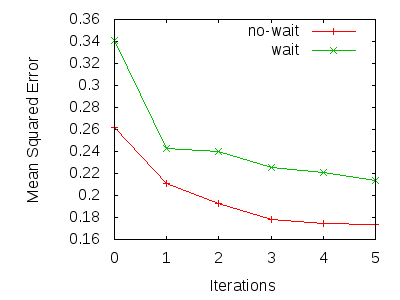
\includegraphics[width=0.7\textwidth]{output.png}
\end{centering}
\label{fig:toyData}
\caption{A toy data example run for LDA formulation}
\end{figure}


\comment{\\ Comparison with PSGD on the speed and accuracy of convergence (Do
we compare on the original objective or the new objective)\\}

\subsection{Qualitative results on latent space models} 
\comment{\\We do both for MMSB and LDA both\\}
\comment{\\Qirong and Alex think that we should include symmetric matrix
factorization as well as it shows the scheduling strategy when thinsg are not cleanly
seperated.}
\section{Results Analaysis and Discussion}

\section{Conclusion}



\bibliography{biblio}
\bibliographystyle{plain}
\end{document}
